\section{Results}
\label{sec:results}

\begin{figure*}[t]
  \centering
  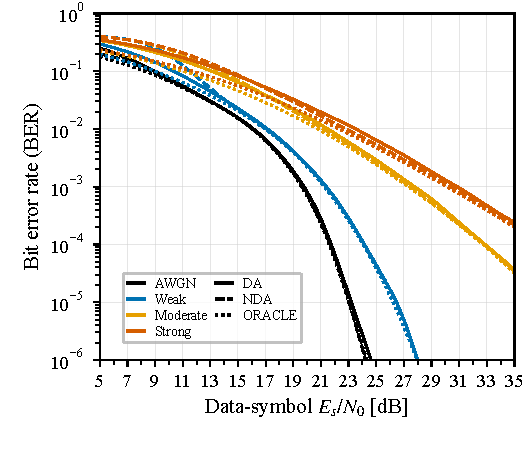
\includegraphics[width=0.78\textwidth]{../../figures/ccisp_fig2_ber.pdf}
  \caption{BER versus average data-symbol SNR for DA-ML, NDA-ML, and the oracle reference under AWGN and five Gamma--Gamma turbulence conditions. Markers denote simulated samples and connecting curves are visual guides. Samples within 5--20~dB (AWGN) and 5--26~dB (turbulence) use 30 seeds with 400 blocks of 256 samples per seed; the high-SNR extension samples use five seeds. The horizontal dash-dotted line marks the $7\%$ HD-FEC reference, $P_b=3.8\times10^{-3}$.}
  \label{fig:ber-overview}
\end{figure*}

\subsection{Simulation and Metric Contract}
\label{sec:simulation-contract}

We evaluate the data-aided (DA) and non-data-aided (NDA) carrier-phase-recovery paths over six channel conditions: an additive white Gaussian noise (AWGN) reference, weak, moderate, and strong downlink Gamma--Gamma turbulence, and moderate and strong uplink turbulence. The benchmark sweep uses 30 independent seeds at every operating point. Each seed contains 400 blocks of 256 received samples, or 102400 samples per operating point. The sampled average data-symbol signal-to-noise ratios (SNRs) span 5--20~dB for AWGN and 5--26~dB for all turbulent conditions. These common samples provide the basis for the fixed-estimator comparison. The selector-recovery count uses a separate fixed-configuration 30-seed data layer covering 29 prescribed points: eight AWGN SNRs and seven SNRs in each of the three downlink regimes.

Figure~\ref{fig:ber-overview} also displays additional high-SNR samples so that the low-BER portions of the curves remain visible. Those extension samples use five independent seeds and extend the AWGN, weak, moderate, and strong/uplink curves to 30, 40, 46, and 50~dB, respectively. Together, the 30-seed benchmark and five-seed extension provide the complete displayed SNR range. Figure~\ref{fig:crossover} uses the same merged curve set, while the selector count is evaluated on its separate fixed-configuration 30-seed grid.

The primary metric is the bit error rate (BER), $P_b$. For NDA, all 256 16-APSK symbols carry data, giving 1024 data bits per block. With one pilot every four symbols, DA is evaluated over the remaining 192 data symbols, giving 768 data bits per block. This data-BER convention evaluates the decoded payload positions of each branch. The $7\%$ hard-decision forward-error-correction (HD-FEC) reference is $P_b=3.8\times10^{-3}$ \cite{takimoto2024modegroup}; Fig.~\ref{fig:ber-overview} uses it as a visual performance reference, while the selector statistics follow the data-BER definition.

\subsection{DA--NDA Behavior}
\label{sec:da-nda-behavior}

Figure~\ref{fig:ber-overview} shows the complementary operating regions of the two estimators. DA uses known pilot symbols to support carrier estimation, whereas NDA preserves all symbol positions for payload. In the predefined work region $\gamma_{\mathrm{tot}}\geq15$~dB, the NDA-versus-DA equivalent-SNR advantage is approximately 1.3~dB for strong downlink turbulence, 1.2~dB for moderate uplink turbulence, and 1.9~dB for strong uplink turbulence. These three values are averages over that work region after expressing the two estimators on the stated total-energy coordinate, which includes the $10\log_{10}(4/3)=1.249387$~dB pilot-energy offset. They report the NDA--DA work-region comparison on a common total-energy coordinate.

The intersections of the DA and NDA data-BER curves provide a second view of this complementarity. Using linear interpolation in log-BER between simulated samples, the observed crossover SNRs are 18.0, 16.9, and 10.7~dB for weak, moderate, and strong downlink turbulence, respectively. Figure~\ref{fig:crossover} marks these post-simulation curve observations directly. The receiver uses one fixed 13~dB effective-SNR decision level shared by all evaluated regimes.

\begin{figure}[t]
  \centering
  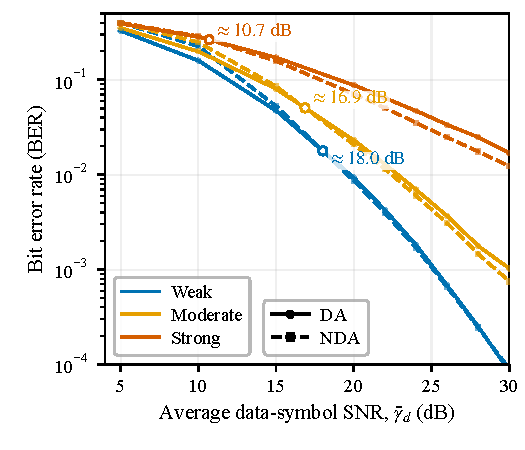
\includegraphics[width=\columnwidth]{../../figures/ccisp_fig4_crossover.pdf}
  \caption{Observed DA--NDA data-BER crossovers for weak, moderate, and strong downlink turbulence. Solid curves with circular samples denote DA, dashed curves with square samples denote NDA, and open circles mark log-BER-interpolated intersections at 18.0, 16.9, and 10.7~dB. The selector applies its shared fixed 13~dB effective-SNR decision level across these regimes.}
  \label{fig:crossover}
\end{figure}

\subsection{Switching Evaluation}
\label{sec:switching-gain}

We quantify the selector relative to a receiver that always uses NDA at the same average data-symbol SNR. For each operating point, the BER-ratio reduction is
\begin{equation}
G_{\mathrm{BER}}=10\log_{10}\!\left(\frac{P_{b,\mathrm{NDA}}}{P_{b,\mathrm{SW}}}\right),
\label{eq:ber-ratio-reduction}
\end{equation}
where $P_{b,\mathrm{NDA}}$ and $P_{b,\mathrm{SW}}$ are the fixed-NDA and switched-path BERs, respectively. A positive $G_{\mathrm{BER}}$ gives the logarithmic BER reduction at a common data-symbol SNR. Figure~\ref{fig:ber-reduction} reports this metric over the three downlink turbulence regimes. Representative positive values are 2.3~dB at 10~dB in weak turbulence, 2.0~dB at 10~dB in moderate turbulence, and 1.3~dB at 5~dB in strong turbulence. These anchors illustrate the reduction obtained when the selector activates the branch favored by its fixed decision rule.

Across the selector grid, 29 operating points are evaluated: eight AWGN SNRs plus seven SNRs in each of the weak, moderate, and strong downlink regimes, i.e., $29=8+7+7+7$. Using the standard data-BER definition to identify the lower-BER fixed estimator, the selector recovers that estimator at 26 of the 29 points. This count and Fig.~\ref{fig:ber-reduction} describe complementary aspects of operation: the count measures branch recovery across the prescribed grid, whereas $G_{\mathrm{BER}}$ measures the BER reduction relative to fixed NDA at each common SNR. Together, they show that a single fixed 13~dB decision level shared across regimes converts the DA--NDA operating-region complementarity into repeatable estimator selection.

\begin{figure}[t]
  \centering
  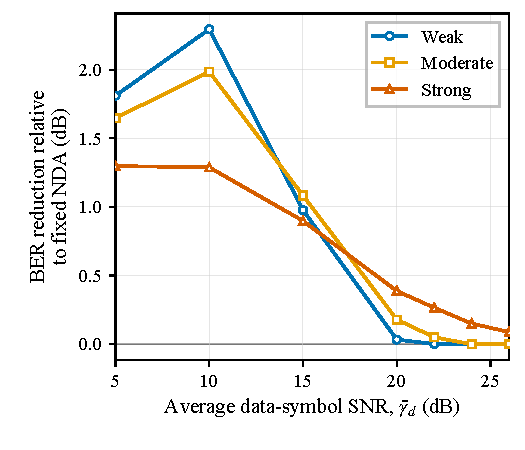
\includegraphics[width=\columnwidth]{../../figures/ccisp_fig3_gain.pdf}
  \caption{Same-SNR BER reduction of the switched path relative to fixed NDA, $G_{\mathrm{BER}}=10\log_{10}(P_{b,\mathrm{NDA}}/P_{b,\mathrm{SW}})$, for weak, moderate, and strong downlink turbulence. Positive values indicate a lower switched-path BER at the same average data-symbol SNR and directly report the logarithmic BER ratio.}
  \label{fig:ber-reduction}
\end{figure}
